\subsection{USB-B}
\label{subsec:USB-B}

Auf der Leiterplatte des PartyMixer's gibt es zwei Komponenten, welche programmiert werden müssen. Der Mikrocontroller und das WiFi-Modul. Um diese zu programmieren braucht es eine entsprechende Schnittstelle, welche mit einer USB-B-Schnittstelle realisiert wird.

Die USB-B-Schnittstelle benötigt nur zwei Kommunikationsleitungen (D+ und D-). Die zu programmierenden Komponenten (ESP32 und ATMega2560) benötigen zusätzliche Steuerleitungen um in einen Programmiermodus zu kommen und statt einem differenziellen Verfahrens ein serielles Verfahren. Deswegen benötigt es einen USB-UART-Converter.

Die beiden Kommunikationsschnittstellen (ATMega2560 und ESP32) benötigen unterschiedlich viele Steuerleitungen, da sie sich im Verfahren zum Aufruf des Download-Boot-Modus unterscheiden. In Tabelle \ref{tab:USB_uC} und \ref{tab:USB_ESP} wird dargestellt, welche Leitungen für das jeweilige Flash-Interface benötigt werden.
%Die USB-B-seitige Schnittstelle wird an den Computer angeschlossen und muss nicht häher betrachtet werden.

\begin{table}[h!]
\center
\begin{tabular}{|c|lcl|c|}
\hline
\textbf{Mikrocontroller} & & & & \textbf{USB-Flash-Device} \\ \hline
RX & <== & direkt & === & TX  \\
TX & === & direkt & ==> & RX  \\
Reset & <== & Kondensator & === & DTR \\
\hline
\end{tabular}
\caption{Verbindung zwischen USB und Mikrocontroller.}
\label{tab:USB_uC}
\end{table}

\begin{table}[h!]
\center
\begin{tabular}{|c|lcl|c|}
\hline
\textbf{ESP} & & & & \textbf{USB-Flash-Device} \\ \hline
RX & <== & direkt & === & TX  \\
TX & === & direkt & ==> & RX  \\
EN & <== & über Transistor & === & RTS \\
IO\_0 & <== & über Transistor & === & DTR \\
IO\_13 & <== & über Widerstand & === & RTS \\
IO\_15 & <== & über Widerstand & === & CTS \\
\hline
\end{tabular}
\caption{Verbindung zwischen USB und ESP.}
\label{tab:USB_ESP}
\end{table}

%Um in den automatischen Programmiermodus zu kommen, muss folgender Handshake zwischen den Geräten stattfinden:


%Auch hier wurde vom Arduino Uno-Board abgekpufert und der selbe Chip verwendet, um die USB-Signale in UART-Signale zu konvertieren. Das vorkommende Bauteil ist der CP2102N. Da dieser Chip ein TQFP-28-Gehause hat, könnte es auch schwierigkeiten geben beim Löten. Deswegen wird auch ein Breakout-Board (BOB) mitgeplant, damit es eine Ausweichmöglickeit gibt falls die Bauteile zu klein sind.

%\begin{figure}[!h]
%\center
%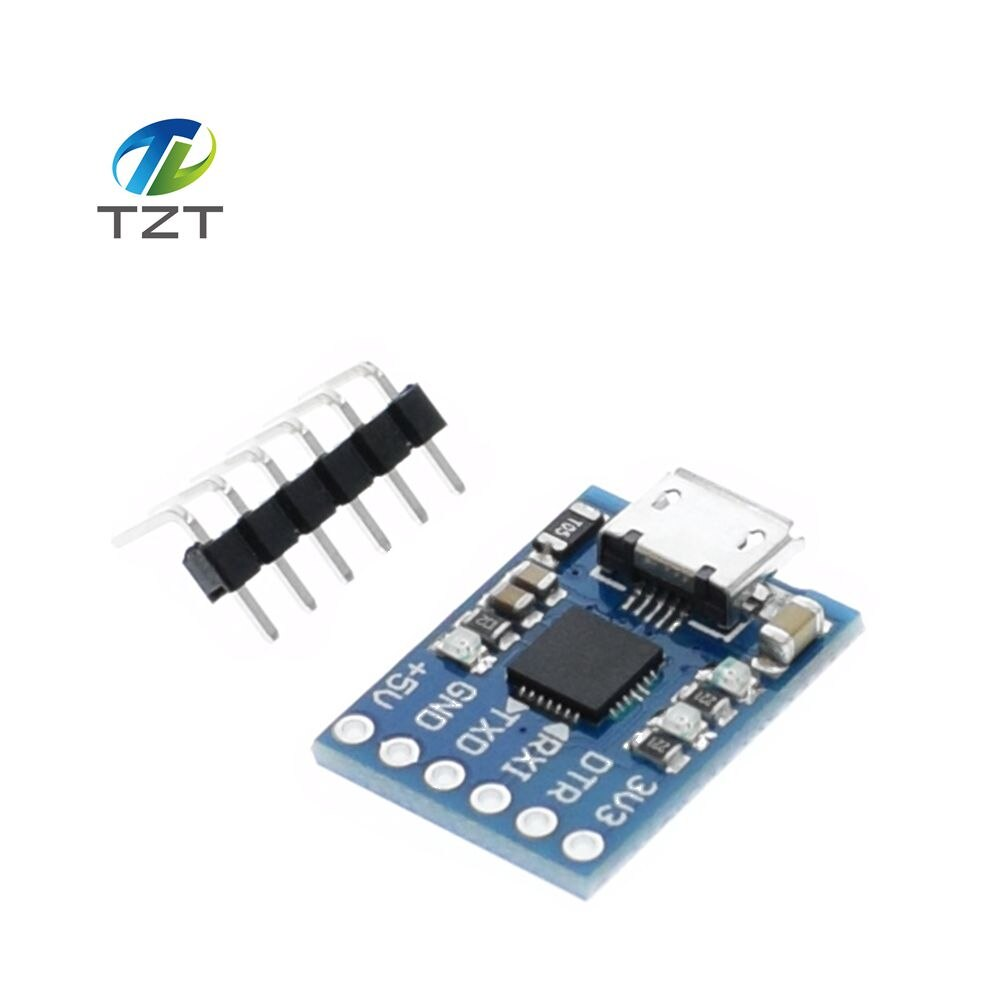
\includegraphics[width = 0.5\textwidth]{graphics/Produktbild_USB_UART_uC}
%\caption{CP2102N-BOB für uC.}
%\label{fig:Produktbild_USB_UART_uC}
%\end{figure}
%
%\begin{figure}[!h]
%\center
%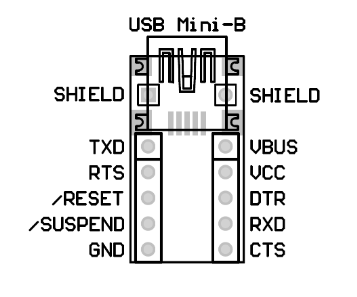
\includegraphics[width = 0.5\textwidth]{graphics/Produktbild_USB_UART_ESP}
%\caption{CP2102N-BOB für ESP.}
%\label{fig:Produktbild_USB_UART_ESP}
%\end{figure}